\documentclass[10pt]{article}
\usepackage{amsmath}
\usepackage{amsfonts}
\usepackage{amssymb}
\usepackage{amsthm}
\usepackage{graphicx}   %Include graphics
\usepackage{float}      %Used to force graphics to stay where I want them to stay
\usepackage{mathrsfs}   %for Fourier transform 'F' symbol \mathscr{F}
\usepackage{hyperref}   %For hyperlinks in the PDF
\usepackage{enumitem}   %so we can have nonIndented lists and enumerations
\usepackage{caption}
\usepackage{subcaption}


\pdfpagewidth 8.5in
\pdfpageheight 11in
\setlength{\oddsidemargin}{-.35in}
\setlength{\textwidth}{7.32in}
\setlength{\topmargin}{-.6in}
\setlength{\textheight}{9.4in}

%%%%%%%%%%%%%%%%%%%%%%%%%%%%%%%%%%%%%%%%%%%%%%%%%%%%%%%%%%

%matrix macro
\newcommand{\mat}[2][ccccccccccccccc]{\left [\!\!\begin{array}{#1} #2\\ \end{array} \!\!\right]}
\newcommand{\determ}[2][ccccccccccccccc]{\left| \begin{array}{#1} #2\\ \end{array} \right| \vspace{.5em}}

%permutation
\newcommand{\perm}[2][ccccccccccccccc]{\left (\begin{array}{#1} #2\\ \end{array} \right) \vspace{.5em}}

%piecewise function
%  example:
%     $$H_i(K, K_0)\iso\piece{ \trivial & \text{if $i=0$} \\ \bbz/2\bbz &\text{if $i=1$} \\ \trivial & \text{if $i\ge2$}}$
%
\newcommand{\piece}[2][cll]{\left \{\begin{array}{#1} #2\\ \end{array} \right. }

%system of equations
\newcommand{\sys}[2][lll]{\left \{\begin{array}{#1}#2 \\ \end{array} \right. }

%integral
\newcommand{\dint}{\displaystyle\int}

%sum
\newcommand{\dsum}[3]{
           \displaystyle\sum_{#1}^{#2} #3 }

%sum start i=0
\newcommand{\dsumiz}[2]{
           \displaystyle\sum_{i=0}^{#1} #2}

%sum start i=1
\newcommand{\dsumio}[3]{
           \displaystyle\sum_{i=1}^{#2} #3 }


%sets {b,...,e} and sets with conditions {x | x is an integer}
\newcommand{\set}[2]{  \left\{#1,\ldots,#2\right\} }
\newcommand{\dset}[2]{  \left\{#1\; :\;\;#2\right\} }
\newcommand{\plist}[2]{  \left(#1,\ldots,#2\right) }

\newcommand{\iso}{\cong}
\newcommand{\abs}[1]{ \left|#1\right|}
\newcommand{\pdfrac}[2]{\!\left(\dfrac{#1}{#2}\right)\! }
\newcommand{\pfrac}[2]{\!\left(\frac{#1}{#2}\right)\! }

\newcommand{\libzptrl}[2]{\dfrac{\partial #1}{\partial #2} }
\newcommand{\plibzptrl}[2]{\left(\dfrac{\partial #1}{\partial #2}\right) }
\newcommand{\libz}[2]{\dfrac{d #1}{d #2} }
\newcommand{\plibz}[2]{\left(\dfrac{d #1}{d #2}\right) }
\newcommand{\eval}[2]{\bigg|_{#1}^{#2}}
\newcommand{\transpose}[1]{{#1}\!^T\!}

\newcommand{\mean}{\mbox{E}}
\newcommand{\var}{\mbox{V}}
\newcommand{\cor}{\mbox{Cor}}

\newcommand{\inn}{^{\mbox{inn}}}
\newcommand{\out}{^{\mbox{out}}}
\newcommand{\innL}{^{\mbox{innL}}}
\newcommand{\innR}{^{\mbox{innR}}}
\newcommand{\outL}{^{\mbox{outL}}}
\newcommand{\outR}{^{\mbox{outR}}}
\newcommand{\iloe}{^{\mbox{iloe}}}
\newcommand{\olie}{^{\mbox{olie}}}
\newcommand{\iloeL}{^{\mbox{iloeL}}}
\newcommand{\iloeR}{^{\mbox{iloeR}}}
\newcommand{\olieL}{^{\mbox{olieL}}}
\newcommand{\olieR}{^{\mbox{olieR}}}
\newcommand{\m}{^{{\mbox{m}}}}
\newcommand{\mL}{^{{\mbox{mL}}}}
\newcommand{\mR}{^{{\mbox{mR}}}}
\newcommand{\comp}{^{{\mbox{c}}}}
\newcommand{\inv}{^{-1}}
\newcommand{\pprime}{^{\prime\prime}}
\newcommand{\erf}{\mbox{Erf}\,}
\newcommand{\Span}{\mbox{span}}

\newcommand{\trivial}{\{0\}}						%trivial group (abelian) {0}
\newcommand{\cbrace}[1]{\left\{#1\right\}}				%curly-braces {parameter}
\newcommand{\gen}[1]{\left\langle#1\right\rangle}
\newcommand{\norm}[1]{\left|\left|#1\right|\right|}
\newcommand{\dsup}[1]{displaystyle{\sup_{#1}}}
\newcommand{\range}{\mathrm{range}\;}
\newcommand{\trace}{\mathrm{trace}\;}
\newcommand{\lcm}{\mathrm{lcm}\;}
\newcommand{\clos}{\mathrm{clos\!}\;}
\newcommand{\supnorm}[1]{\norm{#1}_\infty}
\newcommand{\clin}{\mathrm{clin\!}\;}
\newcommand{\lin}{\mathrm{lin\!}\;}

\newcommand{\tuple }[2]{\left(#1, #2\right)}
\newcommand{\paren}[1]{\!\left(#1\right)\!}
\newcommand{\bracket}[1]{\left[#1\right]}
\newcommand{\inprod}[2]{\left\langle#1,#2\right\rangle}

\renewcommand\Re{\operatorname{Re}}
\renewcommand\Im{\operatorname{Im}}

\newcommand{\degree}{\ensuremath{^\circ}}
\newcommand{\overbar}[1]{\mkern 1.5mu\overline{\mkern-1.5mu#1\mkern-1.5mu}\mkern 1.5mu}
\newcommand{\Lim}[1]{\raisebox{0.5ex}{\scalebox{0.8}{$\displaystyle \lim_{#1}\;$}}}

\newcommand{\argmin}{\operatornamewithlimits{argmin}}

%%%%%%%Boxes%%%%%%%%%%%%%%
\newcommand{\fpbox}[2]{
       \fbox{\parbox{#1}{#2}}
}
\newcommand{\cfbox}[1]{
\begin{center}
       \fbox{#1}
\end{center}
}
%%%%%%%%%%%%%%%%%%%%%%%%%%


%black board font
\newcommand{\bbc}{\mathbb{C}}
\newcommand{\bbd}{\mathbb{D}}
\newcommand{\bbf}{\mathbb{F}}
\newcommand{\bbn}{\mathbb{N}}
\newcommand{\bbz}{\mathbb{Z}}
\newcommand{\bbq}{\mathbb{Q}}
\newcommand{\bbr}{\mathbb{R}}
\newcommand{\bbt}{\mathbb{T}}
\newcommand{\bbx}{\mathbb{X}}
\newcommand{\bbu}{\mathbb{U}}

%script font
\newcommand{\sca}{\mathcal{A}}
\newcommand{\scb}{\mathcal{B}}
\newcommand{\scs}{\mathcal{S}}
\newcommand{\scl}{\mathcal{L}}
\newcommand{\scu}{\mathcal{U}}
\newcommand{\scm}{\mathcal{M}}
\newcommand{\sck}{\mathcal{K}}
\newcommand{\scf}{\mathcal{F}}
\newcommand{\sch}{\mathcal{H}}

\newcommand{\KL}{\mathcal{KL}}

 \renewcommand{\i}{\mathrm{i}}

\newcommand{\tinyspace}{5em }
\newcommand{\mediumspace}{10em }
\newcommand{\largespace}{10em }
\newcommand{\largerspace}{20em }
\newcommand{\hugespace}{40em }
\newcommand{\seperator}{\underline{\hspace{45em}}}

%%%%%%%%%%%%%%%%%%%%%%%%%%%%%%%%%%%%%%%%%%%%%%%%%%%%%%%%%%

%stretch rows of a table
\renewcommand*\arraystretch{1.2} %1.1

\pagestyle{plain}
\begin{document}

    \title{AMS 232 Nonlinear Optimization Hw \#4}
    \author{}
    \date{\today}
    \maketitle

%Problem Set
\begin{enumerate}[leftmargin=*]
\item We consider a double integrator under a friction force where, given an initial position and velocity at time $t_0=0$, we want to drive the system to the origin (position zero and at rest) in minimum time when the control (which is force applied to the particle) is bounded by 1.  In this system, we have state $x= \mat{x\\v}\in\bbr^2$ and a control $u\in\bbr$. The optimal control problem-formulation is given as:
        \begin{align*}
            P_{DIfriction} : \piece{ \text{Minimize} & J[x(\cdot), u(\cdot), t_f] = t_f \\
                    \text{Subject to} & \dot x = \mat{\dot x \\ \dot v} = \mat{v \\ u-v }\triangleq f(x,u) \\
                     & t_0 = 0 \\
                     & x(t_0)=\mat{x^0\\v^0}\in\bbr^2 \\\\
                     & x(t_f)=\mat{0\\0} \\
                     & \abs{u}\le 1
                 }
        \end{align*}
      (\textbf{\S1}): First we formulate the necessary conditions for ($P_{DIfriction}$) by applying Pontryagin's Minimum Principle.  From the problem formulation above we are able to identify all of the necessary problem-data required to apply PMP.  The running-cost, time-invariant, is $F(x,u)=0$, the endpoint cost is only a function of final-time, so $E(t_f)=t_f$, the dynamics are time invariant so we have $f(x,u)=\mat{v \\ u-v }$ and the end-event only being a function of the state at the final time: $e(x(t_f))=\mat{x(t_f)-0\\v(t_f)-0}$. (remember $x(t_f)^T=\mat{x(t_f) & v(t_f)}$)
      \begin{enumerate}[label=\roman*]
        \item Formulate the Control Hamiltonian:  Since $P_{DIfriction}$ is time invariant, we have that
              \begin{align*}
                H(x,\lambda, u) = F(x,u) + \lambda^Tf(x,u) = \lambda_x v + \lambda_v(u-v)
              \end{align*}
              Since the Hamiltonian is time invariant, we have that $\libz{H}{t}=0$.  Therefore for all $t\in[t_0,t_f]$, $H[@t]$ is a constant.
        \item Adjoint Equations: The PMP gives that, necessarily, the costates evolve according to $\dot\lambda = -\libzptrl{H}{x}$, so therefore we have
            \begin{align*}
                \dot\lambda = \mat{\dot\lambda_x \\ \dot\lambda_v }
                            = \mat{-\libzptrl{H}{x} \\[.8em] - \libzptrl{H}{v}}
                            = \mat{0 \\ -\lambda_x + \lambda_v}
            \end{align*}
        \item HMC:  With the box constraint on the control, (i.e.: $\forall t\in[t_0,t_f]\,\,\, \abs{u(t)}\le1$) ,the HMC is given as
                  \begin{equation} \label{eq:p1}
                  \left\{
                        \begin{aligned}
                            & \underset{u}{\text{minimize}}
                            & & H(x,\lambda,u) \\
                            & \text{subject to}
                            & & -1\le u \le 1
                            \end{aligned}
                             \right.
                  \end{equation}
                  Which must be solved for each $t\in[t_0,t_f]$.  Because of the box control constraint, to find the necessary condition on $u$ to solve the HMC problem, we must look to the KKT conditions, and for that we must first construct the Lagrangian of the (control) Hamiltonian:
                    \begin{align*}
                        \overbar H(x,\lambda,u) = H(x, \lambda, u) + \mu^Th(u)
                    \end{align*}
                  By the constraint $-1\le u \le 1$ we have that $h(u)=u$ and the path covector, $\mu$, is one-dimensional. Also, $h^L=-1$ and $h^U$=1 (matching the notation in Ross' text)
                   \begin{align*}
                    \overbar H(x,\lambda,u) = H(x, \lambda, u) + \mu u
                  \end{align*}
                  The KKT conditions give two necessary conditions:
                  \begin{itemize}
                    \item $\libzptrl{\overbar H}{u} = 0$, which gives $\mu = -\lambda_v$
                    \item Complementary Condition, $\mu^\dagger u$, which gives
                            \begin{align*}
                                \mu : \piece{ \le0 & \text{when $u =-1$} \\
                                              \ge0 & \text{when $u = 1$} \\
                                              =0   & \text{when $u\in(-1,1)$} }
                            \end{align*}
                  \end{itemize}

        \item[] The TTC and the HVC require the endpoint Lagrangian $\overbar E$. Since the end-event is of dimension 2, we have that $\nu$, the endpoint covector, is two dimensions; defined as  $\nu^T = \mat{\nu_1 & \nu_2}\in\bbr^2$; we also have, since the endpoint cost is only a function of final-time and that the end-event is only a function of the final state, the endpoint Lagrangian is given as
                \begin{align*}
                    \overbar E(x(t_f), t_f) = E(t_f) + v^Te(x(t_f)) = t_f + \nu_1x(t_f) + \nu_2v(t_f)
                \end{align*}
        \item TTC: Since $x(t_0)$ and $x(t_f)$ are given in the problem formulation, the TTC will not give us any information.
        \item HVC:  Since the final time is free, we expect the $HVC$ to give us some information about the necessary conditions for optimality:
            \begin{align*}
                H[@t_f] = -\libzptrl{\overbar E}{t_f} = -1
            \end{align*}
            Therefore, since for all $t\in[t_0,t_f]$, we know that $H[@t]$ is a constant, the HVC gives us that $H[@t]=-1$
      \end{enumerate}


      (\textbf{\S2}): From the necessary conditions formulated in section one, we show that the optimal control is bang-bang with at most one switch.  Interestingly, when solving the HMC, the control $u$ does not explicitly appear in the problem.  We will show that $\mu$ along with the complimentary condition will give us the optimal control.  The KKT condition in the HMC gave that $\mu(t)=-\lambda_v(t)$ for each instance of time $t\in[t_0,t_f]$, and from the complementary conation $\mu$ will tell us how the optimal control $u$ behaves.  From the TTC we have that $\lambda_x$ is constant for all time (what this constant is, we do not care), and that $\dot\lambda_v = -\lambda_x + \lambda_v$. Using the integrating factor technique, we solve for $\lambda_v$ as $\lambda_v = a(be^t-1)$ where $a$ and $b$ are constants.  Therefore we have $\mu$ as  $\mu(t)=-\lambda_v(t) = \alpha(\beta e^t+1)$ where $\alpha$ and $\beta$ are constants.  From the complementary condition we have that, $\mu\le0$ gives $u=-1$, $\mu\ge0$ gives $u=1$, and $\mu\le0$ gives $u\in(-1,1)$. Since $\mu(t)= \alpha(\beta e^t+1)$, $mu$ is a monotonic function: $\mu\le0$ for some amount of time, $\mu\ge0$ for some amount of time, and $\mu$ is only zero at one instance of time.  Therefore the optimal control switches at most once, based on the signs of $\alpha$ and $\beta$.  Hence, necessarily, the optimal control switches at most once.


      (\textbf{\S3}): Lastly, we simulate $P_{DIfriction}$ where $x(t_0)\mat{1\\-1}$ and verify the necessary conditions.  The MatLab toolbox Dido was used to simulate $P_{DIfriction}$ and obtain the following figures with 128 nodes; verification and analysis is discussed in the captions of each figure, and the code used to produce these plots are attached to the appendix of this document.

      \begin{figure}[H]
            \centering
            \begin{minipage}{.5\textwidth}
              \centering
              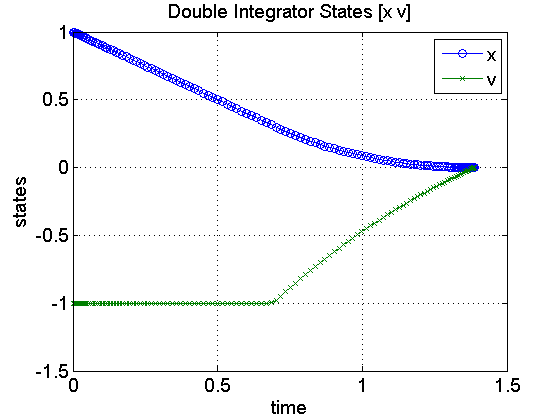
\includegraphics[width=1.\linewidth]{p1states.png}
              \captionsetup{width=0.8\textwidth}
              \captionof{figure}{ State evolution over time to problem $P_{DIfriction}$.  We see that the initial and final states match those given in the problem statement.  }
            \end{minipage}%
            \begin{minipage}{.5\textwidth}
              \centering
              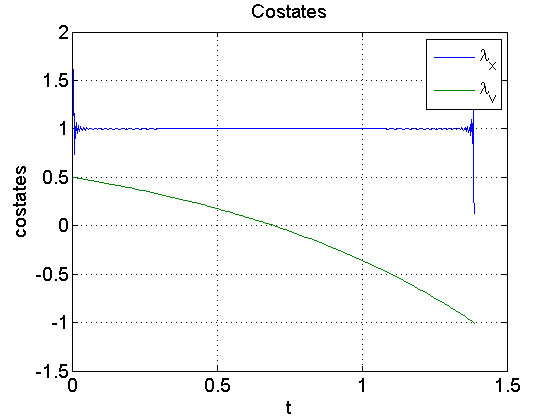
\includegraphics[width=1.\linewidth]{p1costates.png}
              \captionof{figure}{ Evolution of the costates over time to problem to problem $P_{DIfriction}$.  The TTC gives that, necessarily, $\lambda_x$ must be constant for all time, and $\lambda_v$ is an exponential, both of which match the result that Dido returned.}
            \end{minipage}
         \end{figure}

        \begin{figure}[H]
            \centering
            \begin{minipage}{.5\textwidth}
              \centering
              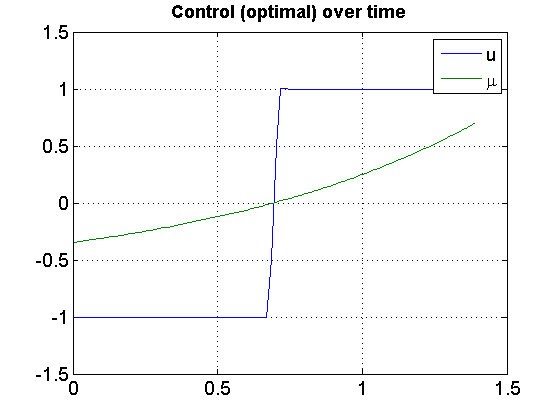
\includegraphics[width=1.\linewidth]{p1control.png}
              \captionsetup{width=0.8\textwidth}
              \captionof{figure}{Evolution of the optimal control over time to problem to problem $P_{DIfriction}$.  We see that $u$ has at most one switch.  Plotted on this figure is $\mu$ from the KKT conditions; we see that when $\mu\le0$, $u=-1$ and when $\mu\ge0$, $u=1$.  The switch occurs at $\mu=0$.  }
            \end{minipage}%
            \begin{minipage}{.5\textwidth}
              \centering
              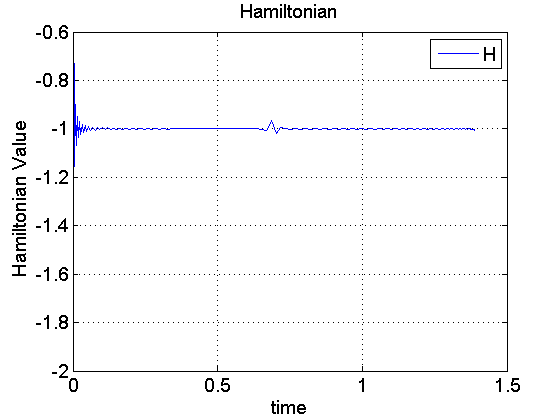
\includegraphics[width=1.\linewidth]{p1hamiltonian.png}
              \captionof{figure}{Evolution of the control Hamiltonian over time to problem to problem $P_{DIfriction}$. The PMP gives that necessarily $H[@t]=-1$ for all time, which is the case for the solution returned by Dido.}
            \end{minipage}
         \end{figure}
        Since the solution returned by Dido satisfies all necessary conditions from the PMP, we expect that this is the optimal solution.

\item Similar to problem 1, given the state $x = \mat{x\\v}\bbr^2$ and the the control $u\in\bbr$, we consider now consider the following $L^1$ optimal control to the double integrator where start and end times are fixed, as are the start and end conditions on the state:
    \begin{align*}
            P_{L^1} : \piece{ \text{Minimize} & J[x(\cdot), u(\cdot), t_f] = \int_{t_0}^{t_f}\abs{u(t)}\,dt \\
                    \text{Subject to} & \dot x = \mat{\dot x \\ \dot v} = \mat{v \\ u }\triangleq f(x,u) \\
                     & t_0 = 0 \\
                     & x(t_0)=\mat{x^0\\v^0}\in\bbr^2 \\\\
                     & x(t_f)=\mat{0\\0} \\
                     & t_f=1\\
                     & \abs{u}\le 6
                 }
    \end{align*}
    (\textbf{\S1}): Because $\abs{u}$ is not smooth, we transfer $P_{L^1}$ to an equivalent formulation with a smooth cost function.  By defining a new control $u = \mat{u_A\\u_B}$ with $u = u_A-u_B$, $\abs{u}=u_A+u_B$, that is, $u_A$ is the positive part of $u$ and $-u_B$ is the negative part of $u$ turned positive.  Therefore a smooth formulation for $P_{L^1}$ is given as
    \begin{align*}
            P_{L^1Mod} : \piece{ \text{Minimize} & J[x(\cdot), u(\cdot), t_f] = \int_{t_0}^{t_f}u_A(t)+u_B(t)\,dt \\
                    \text{Subject to} & \dot x = \mat{\dot x \\ \dot v} = \mat{v \\ u_A-u_B }\triangleq f(x,u) \\
                     & t_0 = 0 \\
                     & x(t_0)=\mat{x^0\\v^0}\in\bbr^2 \\\\
                     & x(t_f)=\mat{0\\0} \\
                     & t_f=1\\
                     & -6\le u_A-u_B\le 6 \\
                     & u_A\ge0 \\
                     & u_B\ge0
                     }
    \end{align*}
    where $u = \mat{u_A\\u_B}$ and $x=\mat{x\\v}$.

    (\textbf{\S2}): We show that $\lambda_v$, the costate associated with state $v$, is linear with respect to time, as well as formulate all of the necessary conditions given by the PMP using the modified formulation, $P_{L^1Mod}$. From the problem formulation above we are able to identify all of the necessary problem-data required to apply PMP.  The running-cost, time-invariant, is only a function of the control, $F(u)=u_A+u_B$, the endpoint cost is given as $E( x(t_f), t_f)=0$, the dynamics are time invariant so we have $f(x,u)=\mat{v \\ u_A-u_B }$ and the end-event $e(x(t_f),t_f)=\mat{x(t_f)-0\\v(t_f)-0\\t_f-1}$.
    \begin{enumerate}[label=\roman*]
        \item Formulate the Control Hamiltonian:  Since $P_{L^1Mod}$ is time invariant, we have that
              \begin{align*}
                H(x,\lambda, u) = F(u) + \lambda^Tf(x,u) = u_A+u_b+\lambda_x v + \lambda_v(u_A-u_B)
              \end{align*}
              Since the Hamiltonian is time invariant, we have that $\libz{H}{t}=0$.  Therefore for all $t\in[t_0,t_f]$, $H[@t]$ is a constant.
        \item Adjoint Equations: The PMP gives that, necessarily, the costates evolve according to $\dot\lambda = -\libzptrl{H}{x}$, so therefore we have
            \begin{align*}
                \dot\lambda = \mat{\dot\lambda_x \\ \dot\lambda_v }
                            = \mat{-\libzptrl{H}{x} \\[.8em] - \libzptrl{H}{v}}
                            = \mat{0 \\ -\lambda_x}
            \end{align*}
            Therefore we see that $\lambda_x$ is a constant for all time, and that $\lambda_v$ is linear for all time.
        \item HMC:  With the box constraint on the control, (i.e.: $\forall t\in[t_0,t_f]\,\,\, \abs{u(t)}\le1$) ,the HMC is given as
                  \begin{equation}
                  \left\{
                        \begin{aligned}
                            & \underset{u}{\text{minimize}}
                            & & H(x,\lambda,u) \\
                            & \text{subject to}
                            & &  u \ge 0 \\
                            &&&   u \ge 0 \\
                            &&&  -6\le u \le 6
                            \end{aligned}
                  \right.
                  \end{equation}
                  Which must be solved for each $t\in[t_0,t_f]$. To find the necessary condition on $u$ to solve the HMC problem, we must look to the KKT conditions, and for that we must first construct the Lagrangian of the (control) Hamiltonian:
                    \begin{align*}
                        \overbar H(x,\lambda,u) = H(x, \lambda, u) + \mu^Th(u)
                    \end{align*}
                  Because of the three constraints, we have that
                  \begin{align*}
                    h(u) = \mat{h_1(u) \\ h_2(u) \\ h_3(u)} = \mat{u_A\\ u_B \\ u_A-u_B}
                  \end{align*}
                  and so as $h:\bbr^2\longrightarrow\bbr^3$, the path covector, $\mu$, is three-dimensional, as $\mu^T=\mat{\mu_1 & \mu_2 & \mu_3}$.  Because of the bounds on each constraint, we have $h_1^L=0, h_2^L=0, h_3^L=-6, h_3^U=6$ (and we can consider $h_1^U,h_2^U=+\infty$).
                   \begin{align*}
                    \overbar H(x,\lambda,u) = u_A+u_b+\lambda_x v + \lambda_v(u_A-u_B) + \mu_1 u_A + \mu_2 u_B + \mu_3(u_A-u_B)
                  \end{align*}
                  And, with $h$ as defined, we can write the HMC compactly as
                  \begin{equation}
                  \left\{
                        \begin{aligned}
                            & \underset{u}{\text{minimize}}
                            & & H(x,\lambda,u) \\
                            & \text{subject to}
                            & &  h^L\le h(u) \ge h^U
                            \end{aligned}
                  \right.
                  \end{equation}

                  The KKT conditions give two necessary conditions:
                  \begin{itemize}
                    \item $\libzptrl{\overbar H}{u} = 0\in\bbr^2$, which gives, since $u$ is now of dimension 2:
                          \begin{align*}
                            \mat{0\\0} = \libzptrl{\overbar H}{u}
                                       = \mat{\libzptrl{\overbar H}{u_A} \\\libzptrl{\overbar H}{u_B} }
                                       = \mat{1+\lambda_v + \mu_1+\mu_3 \\ 1+\lambda_v + \mu_2+\mu_3 }
                          \end{align*}
                    \item Complementary Condition, $\mu^\dagger h(u)$, gives
                            \begin{align*}
                                &\mu_1 : \piece{ \le0 & \text{when $u_A =0$} \\
                                                =0   & \text{when $u_A\in(0,\infty)$} } \\
                                &\mu_2 : \piece{ \le0 & \text{when $u_B =0$} \\
                                                =0   & \text{when $u_B\in(0,\infty)$} } \\
                                &\mu_3 : \piece{ \le0 & \text{when $u_A-u_B =-6$} \\
                                                \ge0 & \text{when $u_A-u_B =6$} \\
                                                =0   & \text{when $u_A-u_B\in(0,\infty)$} }
                            \end{align*}
                          where $\mu_1$ and $\mu_2$ have the $\ge0$ condition taken out since $u_A$ nor $u_B$ are not bounded above.  From the complementary condition, we see the important property that both $\mu_1$ and $\mu_2$ are always non-negative.  Also, these equations are very useful when verifying necessary conditions to your (most likely) computer-generated solutions.
                  \end{itemize}

        \item[iv \& v] The TTC and the HVC give no information for ($P_{L^1Mod}$) as both a full set of initial and final conditions are given on the state (so the TTC will give no information) and the final time is fixed (so the HVC will give no information).  Just for checking, the following is the endpoint Lagrangian:
            \begin{align*}
                \overbar E(x(t_f), t_f) = \nu_1x(t_f) + \nu_2v(t_f) + \nu_3(t_f-1)
            \end{align*}
      \end{enumerate}

    (\textbf{\S3}): Since $\lambda_v$ is linear with respect to time, suppose that $t\in[0,1]$ can be divided into three segments $\Delta^+,\Delta^0,\Delta^-$, where
    \begin{align*}
        \lambda_v(t) : \piece{ >1 & \text{ for $t\in\Delta^+$}\\
                               \in(-1,1) & \text{ for $t\in\Delta^0$}\\
                               <-1 & \text{ for $t\in\Delta^-$}
                       }
    \end{align*}
    Given this, we show that the optimal control $u$ is given by a bang-off-bang controller as
    \begin{align*}
        u(t): \piece{ =-6 & \text{ for $t\in\Delta^+$}\\
                      = 0 & \text{ for $t\in\Delta^0$}\\
                      = 6 & \text{ for $t\in\Delta^-$}
                       }
    \end{align*}
    To solve this problem, we can use the KKT conditions above.  Rather though, let us consider another path.  The HMC of the original problem, $(P_{L^1})$ is
    \begin{equation}
                  \left\{
                        \begin{aligned}
                            & \underset{u}{\text{minimize}}
                            & & H(x,\lambda,u)=\abs{u}+\lambda_xv+\lambda_vu \\
                            & \text{subject to}
                            & & -6\le u \le 6
                            \end{aligned}
                  \right.
    \end{equation}
    And, the goal is to minimize $H$ with respect to $u$, holding $x$ and $\lambda$ constant; that is, $x$ and $\lambda$ are parameters and we are only trying to find $u$ to make $H$ the smallest.  Because adding a constant to a function does not effect where the minimum occurs (i.e.: $\argmin{f(x)}=\argmin{f(x)+k}$ where $k$ is some constant--in words: the location of a/the minimum is not effected by vertical translations), to solve the HMC, we can instead look at the following problem (which will help us solve the problem presented in this section):
    \begin{equation}
                  \left\{
                        \begin{aligned}
                            & \underset{u}{\text{minimize}}
                            & & \hat H(x,\lambda,u)=\abs{u}+\lambda_vu \\
                            & \text{subject to}
                            & & -6\le u \le 6
                            \end{aligned}
                  \right.
    \end{equation}
    Where the hat is on the Hamiltonian is there just to signify that it's not the real Hamiltonian (but finding the $u$ that minimizes $\hat H$ also minimizes $H$).  Now, by the constraint, $-6\le u \le 6$
    \begin{align*}
        &\mbox{When $u>0$, then we have $\hat H = u+\lambda_vu=(\lambda_v +1)u$} \tag{a}\\
        &\mbox{When $u<0$, then we have $\hat H = -u+\lambda_vu=(\lambda_v-1)u$} \tag{b}\\
        &\mbox{When $u=0$, then we have $\hat H = 0$} \tag{c}
    \end{align*}

    For the following three cases, remember we are looking for the value $u$ that minimizes $\hat H$.

    \begin{itemize}
      \item Consider the case when $t\in\Delta^+$, so we know that $\lambda(t)>1$, therefore choosing $u=-6$ minimizes $\hat H$.
      \item Consider the case when $t\in\Delta^-$, so we know that $\lambda(t)<-1$, therefore choosing $u=6$ minimizes $\hat H$.
      \item Consider the case when $t\in\Delta^0$, so we know that $\lambda(t)\in(-1,1)$.  In this case, the choice of $u$ that minimizes $\hat H$ is $u=0$.
    \end{itemize}

    (\textbf{\S4}): Lastly, we simulate $P_{L^1Mod}$, the smooth version, and verify the necessary conditions.  The MatLab toolbox Dido was used to simulate $P_{DIfriction}$ and obtain the following figures with 128 nodes; verification and analysis is discussed in the captions of each figure, and the code used to produce these plots are attached to the appendix of this document.

    \begin{figure}[H]
            \centering
            \begin{minipage}{.5\textwidth}
              \centering
              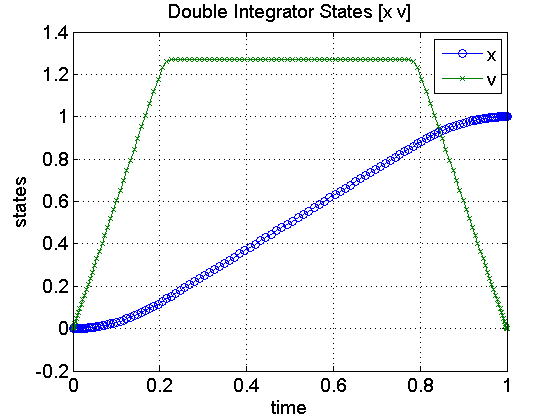
\includegraphics[width=1.\linewidth]{p2states.png}
              \captionsetup{width=0.8\textwidth}
              \captionof{figure}{ State evolution over time to problem $P_{DIfriction}$.  We see that the initial and final states match those given in the problem statement.  }
            \end{minipage}%
            \begin{minipage}{.5\textwidth}
              \centering
              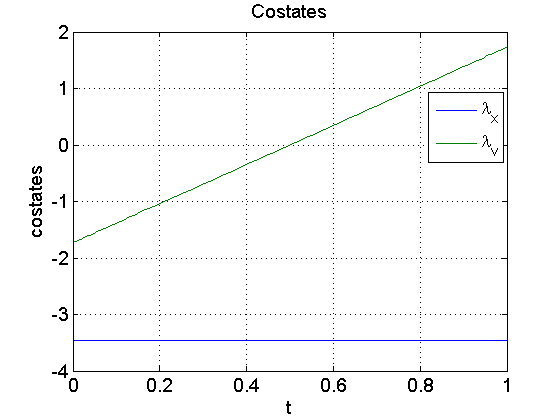
\includegraphics[width=1.\linewidth]{p2costates.png}
              \captionof{figure}{ Evolution of the costates over time to problem to problem $P_{DIfriction}$.  The TTC gives that, necessarily, $\lambda_x$ must be constant for all time, and $\lambda_v$ is linear with respect to time, both of which match the result that Dido returned.}
            \end{minipage}
         \end{figure}

        \begin{figure}[H]
            \centering
            \begin{minipage}{.5\textwidth}
              \centering
              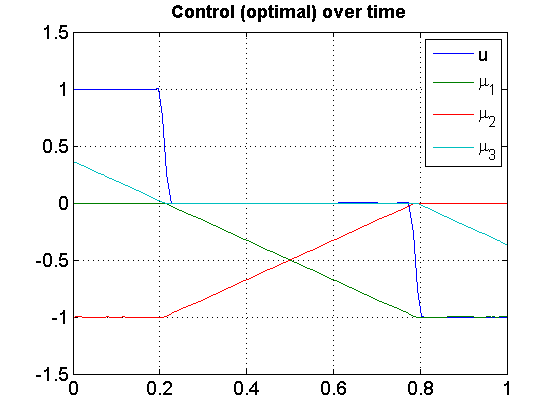
\includegraphics[width=1.\linewidth]{p2control.png}
              \captionsetup{width=0.8\textwidth}
              \captionof{figure}{Evolution of the optimal control over time to problem to problem $P_{DIfriction}$.  We see that $u$ is Bang-Off-Bang.  Plotted on this figure are the time varying KKT covectors $\mu_1,\mu_2,\mu_3$ the complementary condition satisfied.  }
            \end{minipage}%
            \begin{minipage}{.5\textwidth}
              \centering
              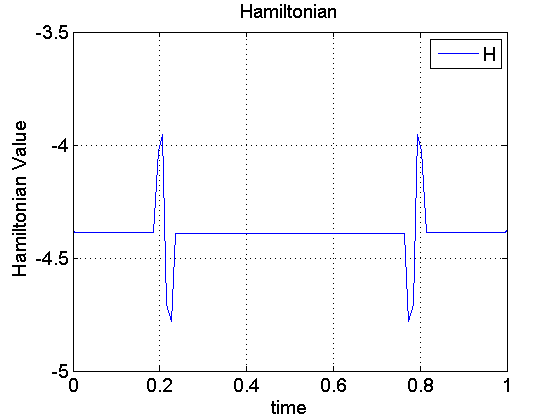
\includegraphics[width=1.\linewidth]{p2hamiltonian.png}
              \captionof{figure}{Evolution of the control Hamiltonian over time to problem to problem $P_{DIfriction}$.  Since the Hamiltonian is time invariant, we have that the Hamiltonian is constant for all time, which is the case for the solution returned by Dido (the blips occur when the control switches).}
            \end{minipage}
         \end{figure}
        Since the solution returned by Dido satisfies all necessary conditions from the PMP, we expect that this is the optimal solution.

\end{enumerate}


\newpage
\subsection*{Matlab Code}{
    To run each problem set, just make a sperate function-file for each function: costFun, dynamicsFun, eventFun, and one script file for the mainProblemFile.m
    \subsection*{Problem1}{
        \begingroup
        \fontsize{7pt}{7pt}
        \begin{verbatim}

function [ endPointCost, runningCost ] = costFun( primal )

    tf = primal.nodes(end);

    endPointCost = tf;
    runningCost = 0;

end


function [ XDot ] = dynamicsFun( primal )

    v = primal.states(2,:); %row vector of size Nx: v(t0)...v(tNn)
    u = primal.controls; %Nu by Nn matrix (hence 1 by Nn for this problem)

    XDot = [ v; u - v ];  %vDot of the brach dynamics
end


function [ endPointConstraints ] = eventFun( primal )

    x0 = primal.states(1,1);
    xf = primal.states(1,end);

    v0 = primal.states(2,1);
    vf = primal.states(2,end);

    endPointConstraints = zeros(4,1);

    endPointConstraints(1) = x0;
    endPointConstraints(2) = v0;
    endPointConstraints(3) = xf;
    endPointConstraints(4) = vf;
end


function [ pathConstraint ] = pathFun( primal )

    pathConstraint = primal.controls;

end


%{
    Implementation of a minimum time double integrator: Section 3.5 of Michael Ross' text:
    A primer on Pontryagin's Principle in Optimal Control

        State x v, where x is position, v is velocity
        Control u represents force, is bounded by -1 and 1 for all time
        Minimize transfer time
        Dynamics  dx = v and dv = u  (where d(.) is time derivative) Dynamics come from
            force=mass*acceleration
        Start at time zero: t0=0
        End time is free
        Object starts with a given position and velocity
        Object must end at position zero at rest
%}
clear all; close all;

Nn = 128;
makeGuess = 0;
loadGuess = 1;
runAccruateMode = 0;

%The Box constraints for the state (x,v)
xL = -20; xU = 20;
vL = -20; vU = 20;

%set the box constraints for the state
bounds.lower.states = [xL; vL];
bounds.upper.states = [xU; vU];


%set the box constraints for the control u. Note: u is unconstrained.
uL = -10; uU = 10;
bounds.lower.controls = [uL];
bounds.upper.controls = [uU];

%Set the constraints on the path function.  hL and hU represent the bounds to the control
%for all time.  We say that for all time hL<=u(t)<=hU
%Note: By setting the control constraints as a path function, we get access to the
%switching function (the time-varying Legrangian value from the Legrange Hamiltonian by
%the KKT conditions)
hL = -1; hU = 1;
bounds.lower.path = [hL];
bounds.upper.path = [hU];


%set the bounds for the initial and final time.  In this problem formulation, the final
%time is free; to do this we allow the final time to be in a range, the upper time (tfMax)
%should be large, but not too large; too large of a horizon could cause your problem to
%fail by falling into some odd local optima pit.
t0 = 0;  tfMax = 100;
bounds.lower.time = [t0; t0];				
bounds.upper.time = [t0; tfMax];

%Set the box constraints for the endpoint constraint (i.e.: 'e' in the problem
%formulation).
x0 = 1; xf = 0;
v0 = -1; vf = 0;
bounds.lower.events = [x0; v0; xf; vf];
bounds.upper.events = bounds.lower.events;   %equality event function bounds


%Note that the path file not required for this problem formulation since the
%problem formulation does not have a path constraint.
linQ.cost 	  = 'costFun';
linQ.dynamics = 'dynamicsFun';
linQ.events	  = 'eventFun';	
linQ.path     = 'pathFun';
linQ.bounds   = bounds;

%To make a guess, we guess the states control and time for the startTime and EndTime
if( makeGuess )
    ourGuess.states(1,:)=[x0, xf];
    ourGuess.states(2,:)=[v0, vf];

    ourGuess.controls(1,:) = [0,0];
    ourGuess.time = [t0, .1*tfMax];

    algorithm.guess = ourGuess;
end

%We can use the primal structure as an initial guess for dido: Eg: Run 20 nodes with the
%made-up guess above and for a run with 32 nodes, we can use the results from the 20 node
%run as a guess to the optimal solution.
if( loadGuess )
    load linQuadPrimal primal;
    algorithm.guess = primal;
end

if( runAccruateMode )
    algorithm.mode = 'accurate';
end

%The number of nodes Nn is Nn+1 sample points taken inbetween the initial and
%final time bounds.  Increase Nn for greater accuracy.
algorithm.nodes = [Nn];

% call dido and record the execution time
tStart= cputime;
    [cost, primal, dual] = dido(linQ, algorithm);
runTime = cputime-tStart;

%%%%%%%%%%%%%%%%%%-----Pretty Plot Code Follows-----%%%%%%%%%%%%%%%%%%

disp(strcat('Dido executed in:', ' ' ,num2str(runTime), ' seconds.'));
disp(strcat('Minimized Cost:', ' ' ,num2str(cost), ' seconds.'));

%Unpack the optimal solution from DIDO's primal structure
xOpt = primal.states(1,:);
vOpt = primal.states(2,:);
uOpt = primal.controls;
tNodes = primal.nodes;

%Optimal Trajectory in the x-v plane
figure;
    plot(xOpt, vOpt);
    title('Phase Plane');
    xlabel('x');
    ylabel('v');
    grid on;

%Plot the control over time along with the switching variable; the Legrangian value from
%the Legrange Hamiltonian.  From the complementary conditions by KKT, we know the
%necessary switching structure the optimal control must have; we know this from the value
%of mu.
figure;
    plot( tNodes, uOpt, tNodes, dual.path);
    title('Control (optimal) over time','fontSize',14,'fontWeight','bold');
    legend('u', '\mu');
    grid on;

%Here we plot the states x v and over time [t0,tf].
figure;
plot(tNodes, xOpt, '-o', tNodes, vOpt, '-x');
    title('Double Integrator States [x v]')
    xlabel('time');
    ylabel('states');
    legend('x', 'v');
    grid on;


%Plot the Control Hamiltonian.
figure;
plot(tNodes, dual.Hamiltonian);
    title('Hamiltonian');
    legend('H');
    xlabel('time');
    ylabel('Hamiltonian Value');
    grid on;


%Plot the costates lambda_x and lambda_v.
figure;
plot(tNodes, dual.dynamics);
    title('Costates')
    xlabel('t');
    ylabel('costates');
    legend('\lambda_x', '\lambda_v');
    grid on;

%Save all variables from the current run with Nn time nodes on [t0,tf].  Note
%that the variable 'primal' can be used as an initial guess.
save linQuadPrimal;

%
% end linQuadProblemFile.m
%
        \end{verbatim}
        \endgroup
    }

    \subsection*{Problem2}{
        \begingroup
        \fontsize{7pt}{7pt}
        \begin{verbatim}
function [ endPointCost, runningCost ] = costFun( primal )

    uA = primal.controls(1,:);
    uB = primal.controls(2,:);

    endPointCost = 0;
    runningCost = uA+uB;

end

function [ XDot ] = dynamicsFun( primal )

    v = primal.states(2,:); %row vector of size Nx: v(t0)...v(tNn)

    uA = primal.controls(1,:);
    uB = primal.controls(2,:);


    XDot = [ v; uA-uB];  %vDot of the brach dynamics
end

function [ endPointConstraints ] = eventFun( primal )

    x0 = primal.states(1,1);
    xf = primal.states(1,end);

    v0 = primal.states(2,1);
    vf = primal.states(2,end);

    endPointConstraints = zeros(4,1);

    endPointConstraints(1) = x0;
    endPointConstraints(2) = v0;
    endPointConstraints(3) = xf;
    endPointConstraints(4) = vf;
end

function [ h ] = pathFun( primal )

    uA = primal.controls(1,:);
    uB = primal.controls(2,:);


    h(1,:) = uA;
    h(2,:) = uB;
    h(3,:) = uA-uB;

end



%{
    Implementation of a minimum time double integrator: Section 3.5 of Michael Ross' text:
    A primer on Pontryagin's Principle in Optimal Control

        State x v, where x is position, v is velocity
        Control u represents force, is bounded by -6 and 6 for all time
        Minimize transfer time
        Dynamics  dx = v and dv = u  (where d(.) is time derivative) Dynamics come from
            force=mass*acceleration
        Start and End time are Fixed
        Object starts with a given position and velocity
        Object must end at a given position at g velocity
%}
clear all; close all;

Nn = 128;
makeGuess = 0;
loadGuess = 1;
runAccruateMode = 0;

%The Box constraints for the state (x,v)
xL = -10; xU = 10;
vL = -10; vU = 10;

%set the box constraints for the state
bounds.lower.states = [xL; vL];
bounds.upper.states = [xU; vU];


%set the box constraints for the control u.  In this formulation we have two controls, uA
%and uB which allows us to smooth out the cost function
uAL = -10; uAU = 10;
uBL = -10; uBU = 10;
bounds.lower.controls = [uAL; uBL];
bounds.upper.controls = [uAU; uBU];

%Set the constraints on the path function.  hL and hU represent the bounds to the control
%for all time.  We say that for all time hL<=u(t)<=hU.  Note that uA>=0 and uB>=0 can also
%be set as box constraints.
hL = -6; hU = 6;
bounds.lower.path = [0;      0;  hL];
bounds.upper.path = [uAU;  uBU;  hU];


%set the bounds for the initial and final time.  In this problem formulation the initial
%and final times are fixed.
t0 = 0;  tf = 1;
bounds.lower.time = [t0; tf];				
bounds.upper.time = bounds.lower.time;

%Set the box constraints for the endpoint constraint (i.e.: 'e' in the problem
%formulation).
x0 = 0; xf = 1;
v0 = 0; vf = 0;
bounds.lower.events = [x0; v0; xf; vf];
bounds.upper.events = bounds.lower.events;   %equality event function bounds


%Note that the path file not required for this problem formulation since the
%problem formulation does not have a path constraint.
linQ.cost 	  = 'costFun';
linQ.dynamics = 'dynamicsFun';
linQ.events	  = 'eventFun';	
linQ.path     = 'pathFun';
linQ.bounds   = bounds;

%To make a guess, we guess the states control and time for the startTime and EndTime
if( makeGuess )
    ourGuess.states(1,:)=[x0, xf];      %Guess for state x
    ourGuess.states(2,:)=[v0, vf];      %Guess for state v

    ourGuess.controls(1,:) = [0, 6];    %Guess for uA
    ourGuess.controls(2,:) = [0, 6];    %guess for uB

    ourGuess.time = [t0, tf];

    algorithm.guess = ourGuess;
end

%We can use the primal structure as an initial guess for dido: Eg: Run 20 nodes with the
%made-up guess above and for a run with 32 nodes, we can use the results from the 20 node
%run as a guess to the optimal solution.
if( loadGuess )
    load linQuadPrimal primal;
    algorithm.guess = primal;
end

if( runAccruateMode )
    algorithm.mode = 'accurate';
end

%The number of nodes Nn is Nn+1 sample points taken inbetween the initial and
%final time bounds.  Increase Nn for greater accuracy.
algorithm.nodes = [Nn];

% call dido and record the execution time
tStart= cputime;
    [cost, primal, dual] = dido(linQ, algorithm);
runTime = cputime-tStart;

%%%%%%%%%%%%%%%%%%-----Pretty Plot Code Follows-----%%%%%%%%%%%%%%%%%%

disp(strcat('Dido executed in:', ' ' ,num2str(runTime), ' seconds.'));
disp(strcat('Minimized Cost:', ' ' ,num2str(cost), ' seconds.'));

%Unpack the optimal solution from DIDO's primal structure
xOpt = primal.states(1,:);
vOpt = primal.states(2,:);
uOpt = primal.controls;
mu = dual.path;
tNodes = primal.nodes;

%Optimal Trajectory in the x-v plane
figure;
    plot(xOpt, vOpt);
    title('Phase Plane');
    xlabel('x');
    ylabel('v');
    grid on;

%Plot the control over time along with the switching variable;
figure;
    plot( tNodes, (1/6)*(uOpt(1,:)-uOpt(2,:)), tNodes, mu);
    title('Control (optimal) over time','fontSize',14,'fontWeight','bold');
    legend('u', '\mu_1', '\mu_2', '\mu_3');
    grid on;

%Here we plot the states x v and over time [t0,tf].
figure;
plot(tNodes, xOpt, '-o', tNodes, vOpt, '-x');
    title('Double Integrator States [x v]')
    xlabel('time');
    ylabel('states');
    legend('x', 'v');
    grid on;


%Plot the Control Hamiltonian.
figure;
plot(tNodes, dual.Hamiltonian);
    title('Hamiltonian');
    legend('H');
    xlabel('time');
    ylabel('Hamiltonian Value');
    grid on;


%Plot the costates lambda_x and lambda_v.
figure;
plot(tNodes, dual.dynamics);
    title('Costates')
    xlabel('t');
    ylabel('costates');
    legend('\lambda_x', '\lambda_v');
    grid on;

%Save all variables from the current run with Nn time nodes on [t0,tf].  Note
%that the variable 'primal' can be used as an initial guess.
save linQuadPrimal;

%
% end linQuadProblemFile.m
%




        \end{verbatim}
        \endgroup
    }

    \subsection*{Problem3}{
        \begingroup
        \fontsize{7pt}{7pt}
        \begin{verbatim}

        \end{verbatim}
        \endgroup
    }
}

\end{document} 